% ============================================================
% 单栏期刊体例（版式参照 examples/paperflow-demo/paper_article.tex）
% 中文排版：ctex + xeCJK，用 tectonic 编译（XeTeX 内核）
%   tectonic -X compile paper.tex
% 正文西文与公式沿用 newtx（Times 系），与中文宋体混排字面高度接近
% ============================================================
\documentclass[11pt,a4paper]{article}

\usepackage[margin=2.5cm]{geometry}
\usepackage{amsmath}

% ---------- 中文 ----------
% fontset=none 后手动指定，避免 tectonic 在无中文字体集时回退成方框
\usepackage[UTF8,fontset=none]{ctex}
\setCJKmainfont{Songti SC}
% 不设 CJK 等宽族：Heiti SC 是 .ttc 集合、fontspec 按族名取不到，
% 而 \url 会切到等宽从而触发查找失败。文中网址改用普通文本，无需等宽。
\setCJKsansfont{Hiragino Sans GB}

% ---------- 西文与数学：Times 系 ----------
\usepackage{newtxtext}
\usepackage{newtxmath}

\usepackage{graphicx}
\usepackage{booktabs}
\usepackage{array}
\usepackage[labelfont=bf,font=small]{caption}
\usepackage[round,semicolon,authoryear]{natbib}
\usepackage{setspace}
\setstretch{1.15}
\usepackage[hidelinks]{hyperref}

% 图表标题用「图 1」「表 1」
\renewcommand{\figurename}{图}
\renewcommand{\tablename}{表}
\renewcommand{\refname}{参考文献}
\captionsetup{labelsep=quad}

\title{\textbf{通向 2030 年的人工智能算力曲线：\\ 外推、约束与最先触及的那堵墙}}
\author{academic-skills / paper-word 示例文稿}
\date{\today}

\begin{document}
\maketitle

\begin{abstract}
\noindent
把“人工智能到 2030 年会走到哪一步”这个问题落到可计算的形式，最直接的代理量是单次训练所投入的算力。本文以两个已发表的量为锚点——训练算力约以每年 4 倍的速度增长、2030 年 $2\times10^{29}$ FLOP 量级的训练很可能可行 \citep{epoch2024}——反推出 2024 年的基准约为 $4.9\times10^{25}$ FLOP，并据此给出 2000—2030 年的算力轨迹。在此基础上，本文把电力、芯片产能、数据存量与延迟墙四类约束放在同一坐标轴上比较，指出它们各自允许的上限相差三个数量级以上，因而“会不会撞墙”这个问句必须被替换成“先撞哪一堵”。

本文进一步把计算最优配比 \citep{hoffmann2022} 与公开人类文本存量的估计 \citep{villalobos2024} 联立，得到一个此前未被并置讨论的结果：在严格等比例配比下，训练 token 数在 $C \approx 2.7\times10^{28}$ FLOP 处即触及约 $3\times10^{14}$ token 的公开文本存量，该点仅为 $2\times10^{29}$ 目标的 0.14 倍。换言之，若不引入合成数据、多模态语料或数据效率的改进，数据侧的紧约束会比电力侧提前约一年半到两年出现。敏感性分析显示，2030 年的结果对年增速极为敏感：年增 4.0 倍对应 $2\times10^{29}$，降到 3.0 倍则只有 $3.6\times10^{28}$，升到 5.1 倍才触及芯片产能的中位上限。

本文的结论不是一条预测曲线，而是一组条件命题：外推本身不构成预测，它只是把各方已发表的判断放进同一套单位里，让分歧显形。
\end{abstract}

\medskip
\noindent\textbf{关键词：} 训练算力；标度律；算力外推；数据存量；约束分析

\begin{center}\fbox{\parbox{0.92\linewidth}{\small\itshape
本文为版式与方法演示文稿。所有外部数值均标注来源并经核对；由这些数值推导出的量（2024 年基准、数据墙位置、敏感性区间）为本文的算术结果，不代表任何机构的官方预测。}}\end{center}

\section{引言}

关于人工智能的未来，公开讨论里最缺的不是观点而是共同的单位。“能力会不会继续提升”“会不会遇到瓶颈”这类问句无法证伪，因为双方对“能力”与“瓶颈”的度量并不一致。一个可操作的替代是把问题收窄到单次训练所投入的算力 $C$：它有明确的单位（FLOP），有公开的历史序列，并且通过标度律与模型规模、数据量建立了定量联系 \citep{kaplan2020,hoffmann2022}。收窄的代价是显然的——算力不等于能力，本文第 5 节会回到这一点——但收窄之后，分歧至少变得可以计算。

算力增长的历史被划分为若干时期。2010 年之前，训练算力大致与摩尔定律同步，倍增周期约 20 个月；深度学习兴起之后，倍增周期缩短到约 6 个月；2015 年前后又出现了一批算力需求高出一到两个数量级的大规模模型 \citep{sevilla2022}。这一加速并非硬件单方面的贡献，而是硬件、资本投入与工程并行度共同作用的结果，因此它不像摩尔定律那样有明确的物理下限可依。

本文要做的是三件事。第一，把外推建立在已发表的锚点上，而不是自选起点，使轨迹可被复核。第二，把四类物理与资源约束换算成同一单位下的上限，看它们的相对位置。第三，把计算最优配比与数据存量估计联立，定位数据侧约束真正开始咬合的算力水平。这三件事都不需要新数据，只需要把已有的数字放进同一套坐标里——而这恰恰是当前讨论中最少被做的一步。

\section{方法}

\subsection{算力、参数与数据的基本关系}

对以 Transformer 为主的稠密模型，训练算力可用参数量 $N$ 与训练 token 数 $D$ 近似表示：
\begin{equation}
C \;\approx\; 6\,N\,D .
\end{equation}
系数 6 来自前向与反向传播中每个参数每个 token 的乘加次数计数。式 (1) 的作用是把三个可观测量绑在一起：给定其中两个即可推出第三个。

\citet{hoffmann2022} 通过训练四百余个模型给出的结论是，在算力预算固定时，$N$ 与 $D$ 应当等比例放大。结合式 (1)，这意味着
\begin{equation}
N_{\mathrm{opt}} \;=\; N_0\left(\frac{C}{C_0}\right)^{1/2},
\qquad
D_{\mathrm{opt}} \;=\; D_0\left(\frac{C}{C_0}\right)^{1/2},
\end{equation}
其中 $(N_0, D_0)$ 取该文报告的 Chinchilla 配置：$N_0 = 7\times10^{10}$、$D_0 = 1.4\times10^{12}$，对应 $C_0 = 6N_0D_0 \approx 5.9\times10^{23}$ FLOP。该配置的 token 与参数之比为 $D_0/N_0 = 20$，本文后续沿用这一比例。

\subsection{外推模型与锚点的选取}

设年增倍数为 $g$，则从基准年 $t_0$ 出发的算力轨迹为
\begin{equation}
C(t) \;=\; C(t_0)\, g^{\,t-t_0},
\qquad\text{等价地}\qquad
\log_{10} C(t) \;=\; \log_{10} C(t_0) + (t-t_0)\log_{10} g .
\end{equation}
式 (3) 在对数坐标下是直线，这也是图~\ref{fig:trend} 中各段呈折线的原因：折点即倍增周期发生变化之处。

本文不自行选取历史起点。外推的两个锚点都取自 \citet{epoch2024}：其一是年增倍数 $g = 4.0$（对应倍增周期约 6 个月），其二是 2030 年 $2\times10^{29}$ FLOP 的训练“很可能可行”。由这两个量反推基准年：
\begin{equation}
C_{2024} \;=\; \frac{C_{2030}}{g^{6}} \;=\; \frac{2\times10^{29}}{4^{6}} \;\approx\; 4.9\times10^{25}\ \mathrm{FLOP}.
\end{equation}
这个反推值与该报告另一处独立陈述——已有逾三十个模型达到 $10^{25}$ FLOP 量级——在数量级上相容，可作为一致性校验。需要说明的是，图~\ref{fig:trend} 中 2024 年之前的两段是按已发表的倍增周期反推出的轨迹，不是逐模型的实测散点；它们用于呈现折点的位置，不用于宣称任何单一模型的算力。

\subsection{约束的换算口径}

四类约束的上限直接引自 \citet{epoch2024}，均已换算为“该约束单独作用时 2030 年所允许的单次训练算力”。电力约束区分两种部署形态：单一园区受限于本地电网接入，跨地域分布式训练则可汇集更大功率但要付出通信代价。芯片产能以 H100 等效卡数计量。数据约束以多模态有效 token 数计量，与仅计文本的存量估计口径不同，这一差别在第 4 节讨论。

\section{结果}

\subsection{算力轨迹}

图~\ref{fig:trend} 给出 2000—2030 年的算力轨迹。三段的斜率差异是全图唯一需要读取的信息：2010 年前后倍增周期由约 20 个月缩短到约 6 个月，在对数坐标上表现为斜率增大约 3.3 倍。2024 年之后的虚线段是维持 $g=4.0$ 的外推，终点即锚点二。

\begin{figure}[htbp]
\centering
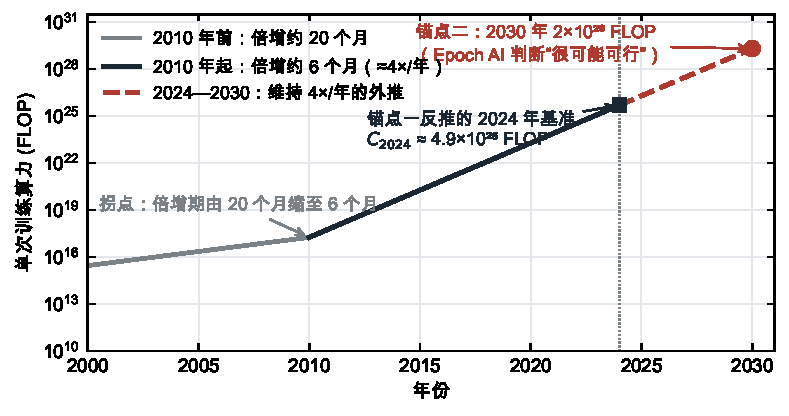
\includegraphics[width=\linewidth]{figures/fig_trend.pdf}
\caption{按已发表的倍增周期与 2030 年结论构造的训练算力轨迹。2024 年前两段为按 \citet{sevilla2022} 的倍增周期反推的轨迹，非逐模型实测点；虚线段为维持年增 4 倍的外推，终点取自 \citet{epoch2024}。}
\label{fig:trend}
\end{figure}

\subsection{四类约束的相对位置}

图~\ref{fig:ceilings} 把四类约束放在同一对数坐标上。三点值得注意。

第一，四条区间的跨度极不对称。电力（单一园区）的上限区间为 $1\times10^{28}$ 至 $3\times10^{29}$ FLOP，而延迟墙为 $3\times10^{30}$ 至 $1\times10^{32}$ FLOP，两者中位相差约两个半数量级。把“AI 会遇到物理瓶颈”当作单一命题讨论，在这个尺度差面前是没有内容的。

第二，综合结论 $2\times10^{29}$ 落在电力（单一园区）区间的上四分之一处，却低于芯片产能区间的下沿 $1\times10^{29}$ 之上不多。这与该报告“最先咬合的是电力，其次是芯片产能”的判断一致 \citep{epoch2024}。

第三，数据与延迟两项的下沿都显著高于综合结论，意味着在 2030 年的时间尺度上它们不是紧约束——但这一判断依赖于“多模态有效 token”的口径，下一节将说明改用纯文本口径后结论会反转。

\begin{figure}[htbp]
\centering
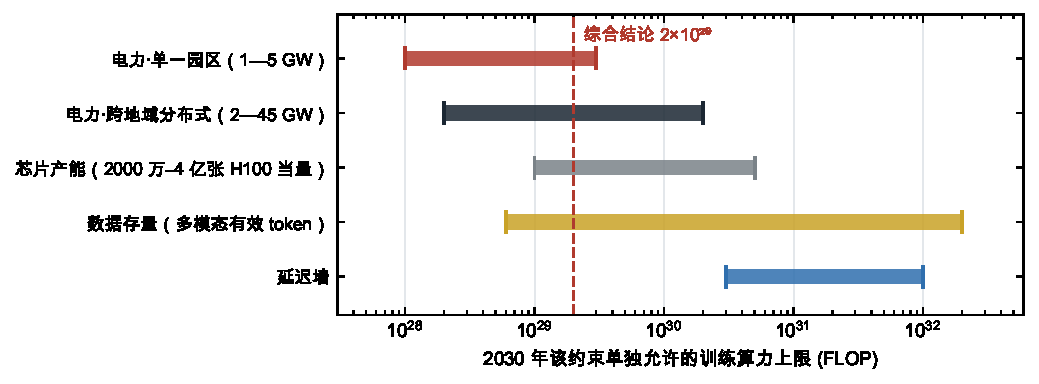
\includegraphics[width=\linewidth]{figures/fig_ceilings.pdf}
\caption{四类约束单独作用时 2030 年所允许的训练算力上限。区间端点均取自 \citet{epoch2024}；虚线为该报告的综合结论 $2\times10^{29}$ FLOP。}
\label{fig:ceilings}
\end{figure}

表~\ref{tab:ceilings} 列出对应数值，便于逐项核对。

\begin{table}[htbp]
\centering
\caption{四类约束的量化上限（数据来源：\citealp{epoch2024}）}
\label{tab:ceilings}
\small
\begin{tabular}{@{}l l l@{}}
\toprule
约束 & 资源口径 & 允许的训练算力 / FLOP \\
\midrule
电力（单一园区） & 1--5 GW & $1\times10^{28}$ -- $3\times10^{29}$ \\
电力（跨地域分布式） & 2--45 GW & $2\times10^{28}$ -- $2\times10^{30}$ \\
芯片产能 & 2\,000 万 -- 4 亿张 H100 等效 & $1\times10^{29}$ -- $5\times10^{30}$ \\
芯片产能（中位） & 1 亿张 H100 等效 & $9\times10^{29}$ \\
数据存量 & $4\times10^{14}$ -- $2\times10^{16}$ 有效 token & $6\times10^{28}$ -- $2\times10^{32}$ \\
延迟墙 & 现有硬件 & $3\times10^{30}$ -- $1\times10^{32}$ \\
\midrule
综合结论 & --- & $2\times10^{29}$ \\
\bottomrule
\end{tabular}
\end{table}

\subsection{数据墙的位置}

把式 (2) 与公开人类文本存量的估计联立，可以定位数据侧约束开始咬合的算力水平。\citet{villalobos2024} 估计公开可得的人类生成文本存量约为 $3\times10^{14}$ token，并预计在 2026—2032 年间被用尽。令 $D_{\mathrm{opt}} = 3\times10^{14}$，由式 (2) 解出
\begin{equation}
C_{\mathrm{data}} \;=\; C_0\left(\frac{D_{\mathrm{data}}}{D_0}\right)^{2}
\;=\; 5.9\times10^{23}\times\left(\frac{3\times10^{14}}{1.4\times10^{12}}\right)^{2}
\;\approx\; 2.7\times10^{28}\ \mathrm{FLOP}.
\end{equation}

这个结果值得停一下。$2.7\times10^{28}$ 仅为综合结论 $2\times10^{29}$ 的 0.14 倍；按 $g=4.0$ 折算，两者相差约 1.4 年。也就是说，在严格等比例配比、且只使用公开人类文本的前提下，数据侧的紧约束会比电力侧提前一年半左右出现——这与图~\ref{fig:ceilings} 中“数据不是紧约束”的印象相反。

两者并不矛盾，差别全在口径。图~\ref{fig:ceilings} 采用的是多模态有效 token（$4\times10^{14}$ 至 $2\times10^{16}$），把图像、音频、视频以及经过质量加权的重复利用都计入；式 (5) 采用的是纯文本存量。结论因此可以精确地表述为：\emph{纯文本路线在 $2.7\times10^{28}$ FLOP 附近失效，继续放大必须依赖多模态语料、合成数据或数据效率的改进。}这三条出路各自的可行性超出本文范围，但它们从“可选项”变成“必需项”的时点，由式 (5) 给出。

\begin{figure}[htbp]
\centering
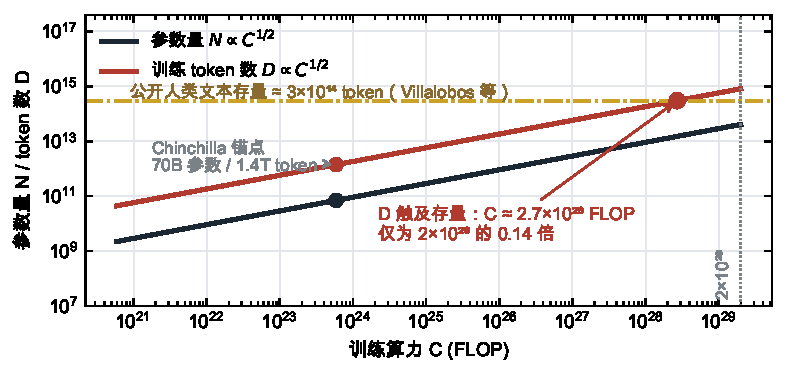
\includegraphics[width=\linewidth]{figures/fig_scaling.pdf}
\caption{计算最优配比下参数量与训练 token 数随算力的走向。锚点为 \citet{hoffmann2022} 报告的 Chinchilla 配置；水平点划线为 \citet{villalobos2024} 估计的公开人类文本存量。两线交点即式 (5) 的 $C_{\mathrm{data}}$。}
\label{fig:scaling}
\end{figure}

\subsection{对增速的敏感性}

2030 年的结果几乎完全由能否维持增速决定。图~\ref{fig:sensitivity} 以 $C_{2024}$ 为起点，横轴取 2024—2030 年持续保持的年增倍数 $g$，纵轴为
\begin{equation}
C_{2030}(g) \;=\; C_{2024}\, g^{6} .
\end{equation}
六次方使结果对 $g$ 极度敏感：$g=3.0$ 时 $C_{2030} \approx 3.6\times10^{28}$，不足综合结论的五分之一；$g=4.0$ 时恰为 $2\times10^{29}$；$g=4.28$ 触及电力（单一园区）上限 $3\times10^{29}$；$g=5.14$ 触及芯片产能中位 $9\times10^{29}$。$g$ 变动四分之一，2030 年的结果变动一个数量级。

因此，对 2030 年状态的任何断言，实质上都是对“年增速能否维持六年”的断言。历史上该增速已维持十余年 \citep{sevilla2022}，但维持它所依赖的资本投入与电力扩张在 2024 年之后进入了新的量级，历史外推的适用性正在减弱。

\begin{figure}[htbp]
\centering
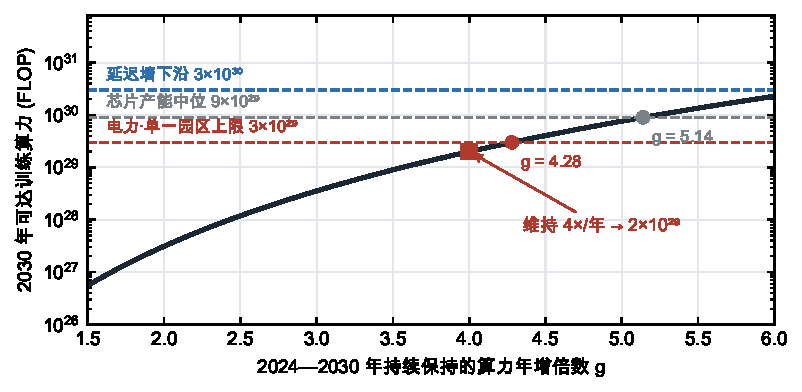
\includegraphics[width=\linewidth]{figures/fig_sensitivity.pdf}
\caption{2030 年可达训练算力对持续年增倍数的敏感性。曲线由式 (6) 计算，起点为式 (4) 的 $C_{2024}$；三条水平虚线为 \citet{epoch2024} 给出的约束上限。}
\label{fig:sensitivity}
\end{figure}

\subsection{约束的物理载体}

前述约束不是抽象的参数，它们对应具体的基础设施。电力约束的载体是数据中心的供电与散热能力（图~\ref{fig:datacenter}）：1--5 GW 的园区级功率相当于一座中型核电机组的输出，其接入周期由电网规划而非芯片供应决定，这正是它最先咬合的原因。芯片产能的载体是先进制程晶圆厂（图~\ref{fig:fab}）：单座厂的建设周期以年计，且受限于光刻设备的交付节奏，产能无法在需求出现后的一两年内响应。

\begin{figure}[htbp]
\centering
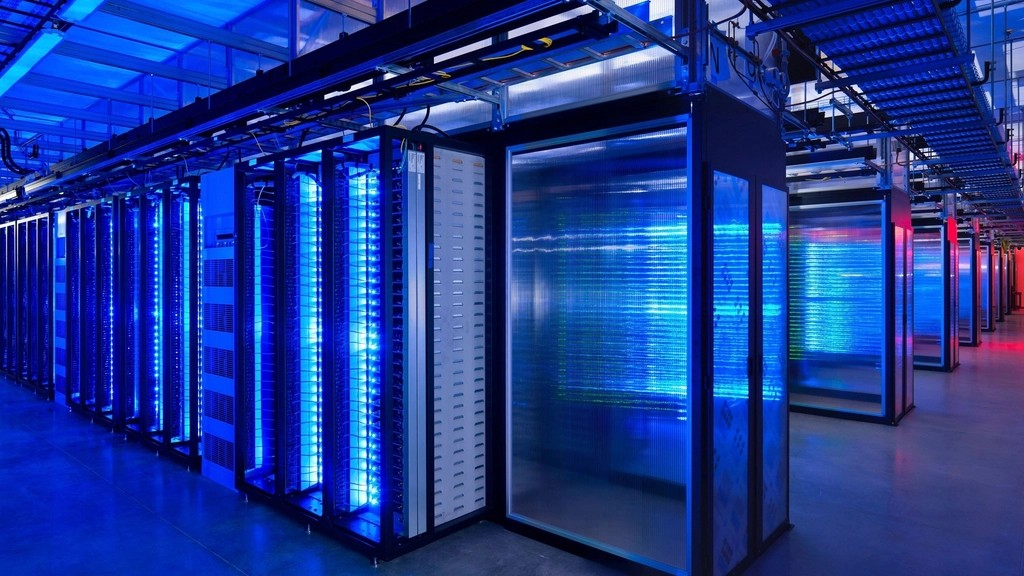
\includegraphics[width=0.72\linewidth]{figures/data_center_server_room_2.jpg}
\caption{数据中心机房。电力接入与散热能力构成本文分析中最先咬合的约束。图片来源：Free computer server room image，CC0。}
\label{fig:datacenter}
\end{figure}

\begin{figure}[htbp]
\centering
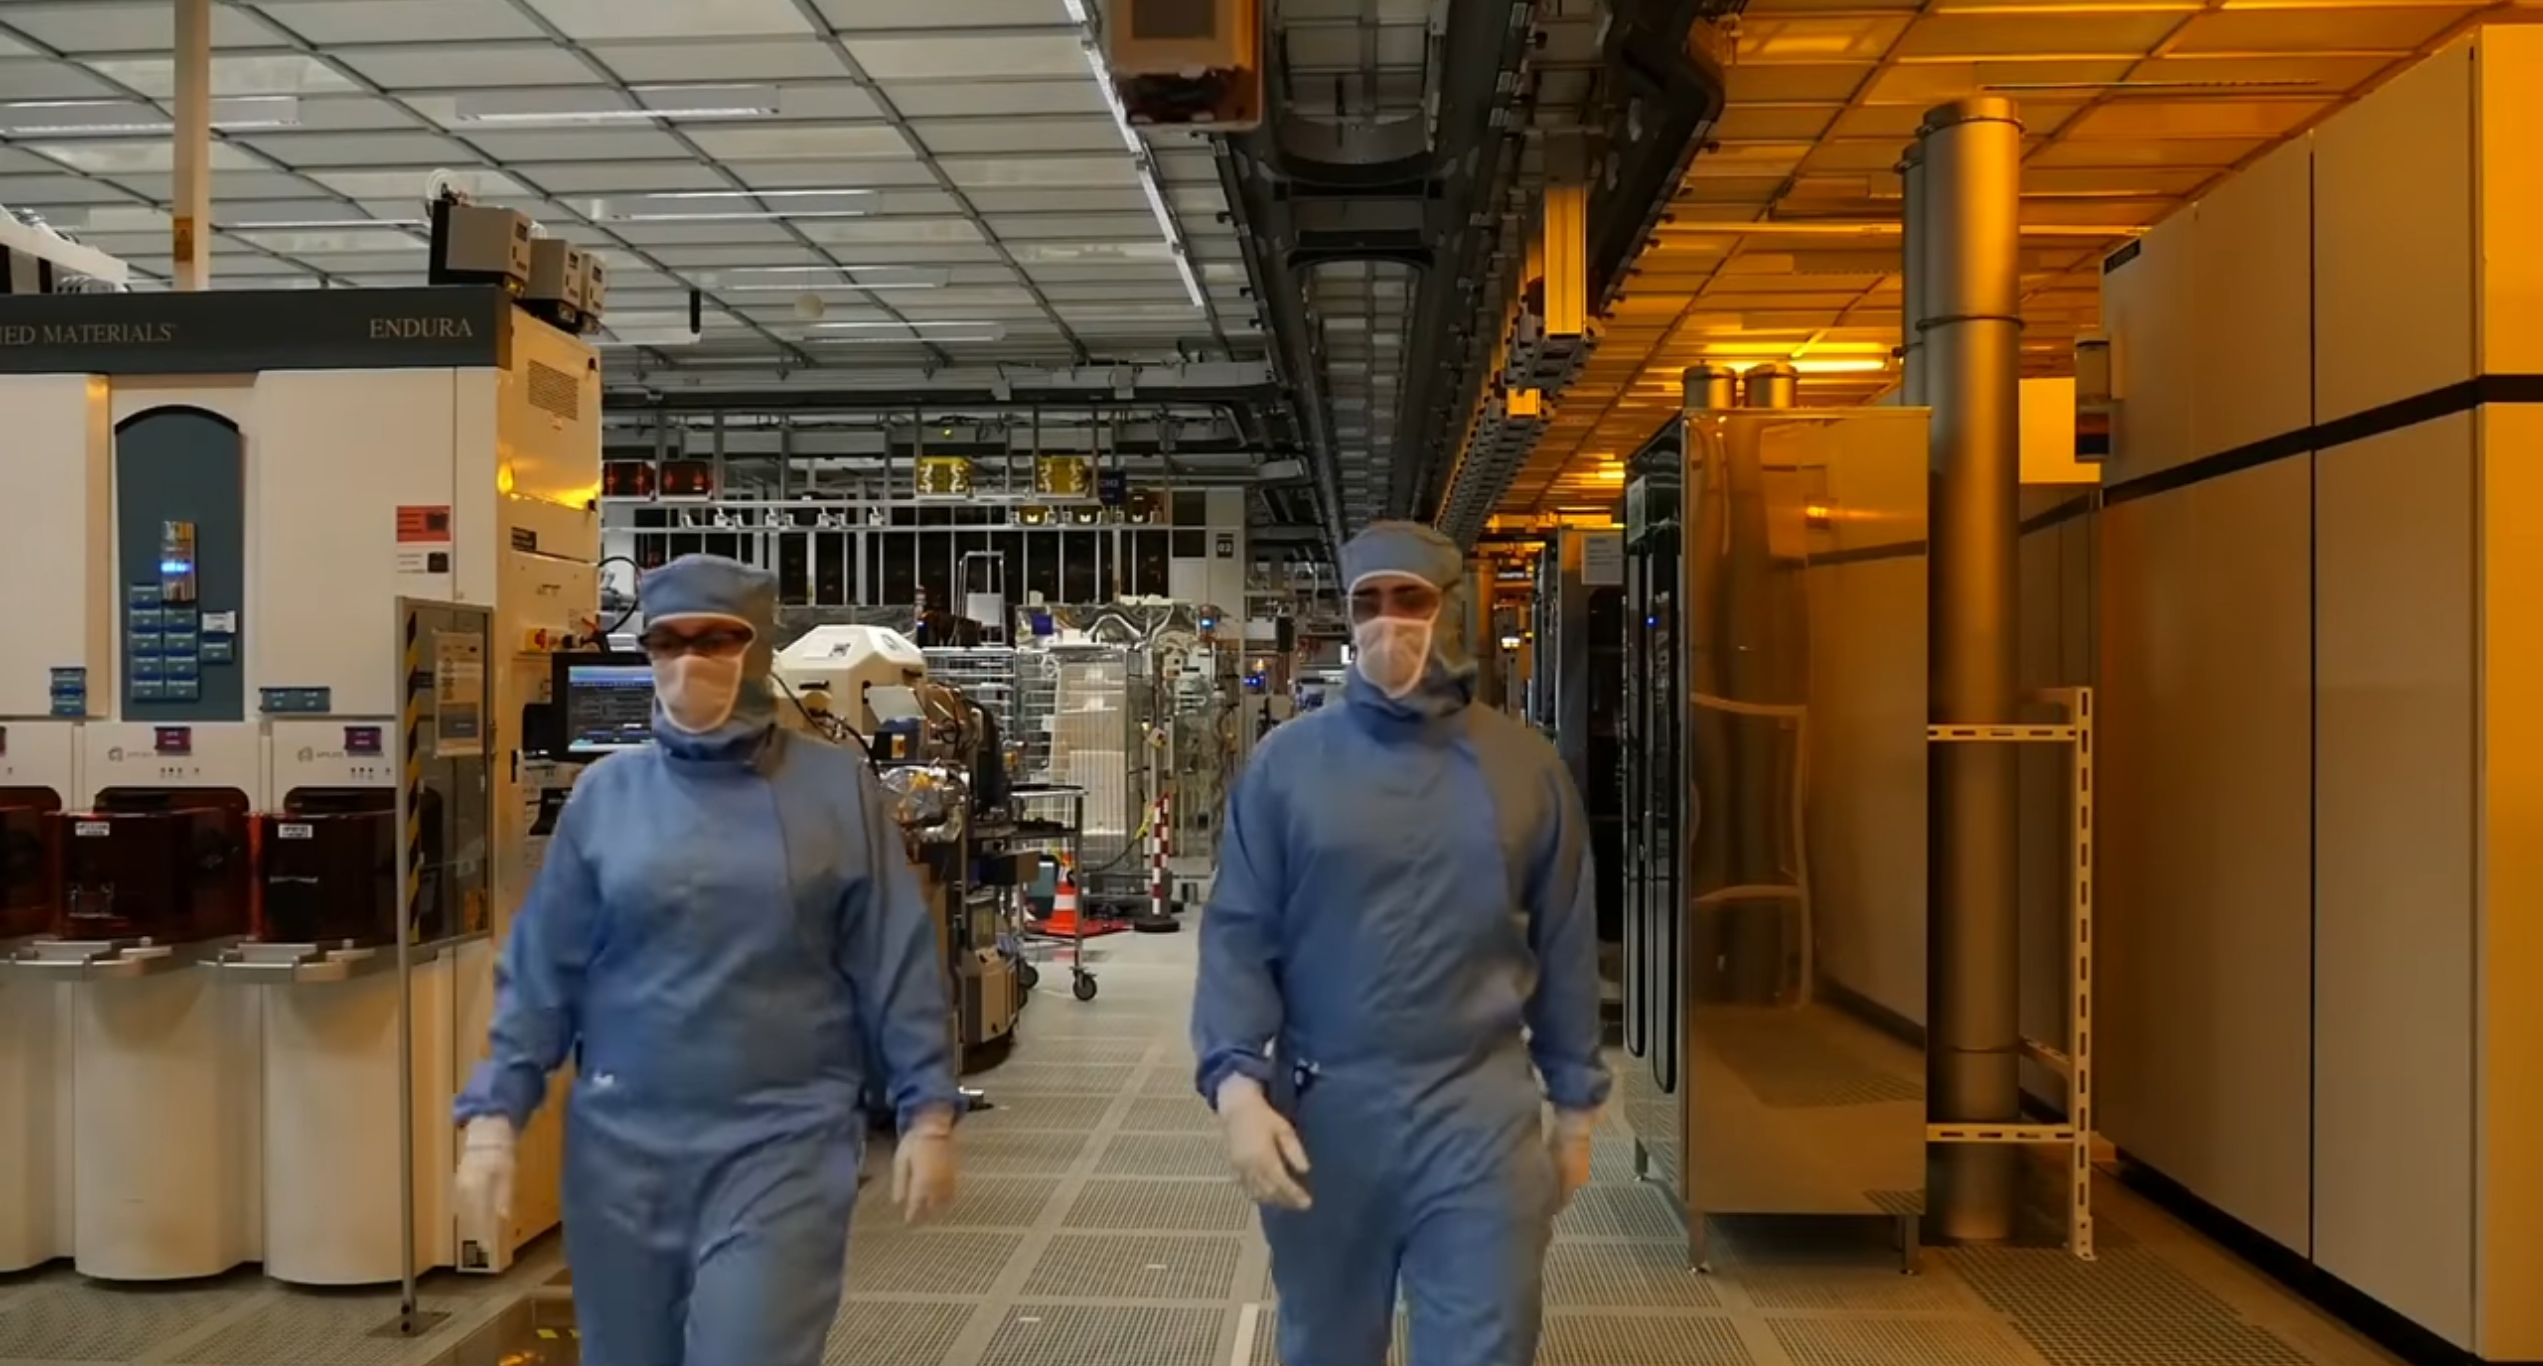
\includegraphics[width=0.72\linewidth]{figures/semiconductor_cleanroom_1.png}
\caption{半导体晶圆厂洁净室。芯片产能是本文分析中第二紧的约束，其扩张周期以年计。图片来源：STMicroelectronics，CC BY。}
\label{fig:fab}
\end{figure}

\section{讨论}

\subsection{外推能承担什么，不能承担什么}

式 (3) 的外推没有内生机制：它不解释增长为何发生，也就无法预告增长何时停止。它能承担的只有一件事——在给定增速假设下，把不同来源的判断折算到同一时间轴上，使分歧可以定位。本文第 3.4 节的敏感性分析正是这一用途的直接体现：与其争论 2030 年的绝对水平，不如争论 $g$ 能否维持，后者是一个更可讨论的问题。

约束分析补上了外推缺失的那一半。指数曲线本身没有上界，而图~\ref{fig:ceilings} 中的四条区间给出了上界的位置。真实轨迹应当是两者的下包络：在触及最紧约束之前近似指数，之后转为受该约束支配的更慢增长。本文没有给出这一转折之后的函数形式，因为它取决于约束被突破还是被绕开，而这属于工程与政策问题，不是外推问题。

\subsection{算力不等于能力}

本文全程以算力为代理量，这个选择的局限必须写明。算力与下游能力之间隔着两层：一是算力到损失的标度律 \citep{kaplan2020,hoffmann2022}，二是损失到具体任务表现的映射。第一层有稳定的幂律形式，但幂指数意味着收益递减——算力提高一个数量级，损失的改善远小于一个数量级。第二层则更不稳定：同一损失水平下，不同任务的表现差异可以很大，且推理时计算的引入进一步削弱了训练算力与最终能力之间的对应关系。

因此，$2\times10^{29}$ FLOP 这个数字所支撑的陈述只能是“规模上的增长空间”，而非“能力上的必然提升”。\citet{epoch2024} 本身也把结论表述为“规模差距相当于 GPT-2 到 GPT-4 之间的差距”，这是一个关于规模的类比，不是关于能力的承诺。

\subsection{三处主要不确定性}

第一，锚点的不确定性。$C_{2024}$ 由式 (4) 反推而来，其精度完全继承自两个锚点。若实际年增速为 3.5 倍而非 4.0 倍，则 $C_{2024}$ 应为 $1.2\times10^{26}$ 而非 $4.9\times10^{25}$，相差 2.4 倍。本文选择反推而非自选起点，是为了让这一继承关系显式可见。

第二，配比假设的不确定性。式 (2) 假定严格的等比例配比，但实际训练常因推理成本考量而偏离——在参数量上让步、在 token 数上加码，可使部署更经济 \citep{hoffmann2022}。这类偏离会使式 (5) 的 $C_{\mathrm{data}}$ 提前到来，即数据墙比本文估计的更早。

第三，口径的不确定性。第 3.3 节已说明纯文本与多模态两种口径给出方向相反的结论。本文的处理是把两者都列出并说明差别，而不是择一。读者若关心的是纯语言模型路线，应以式 (5) 为准；若关心的是包含视觉与音频的通用模型，则图~\ref{fig:ceilings} 的口径更合适。

\section{结论}

本文把关于 2030 年人工智能规模的讨论收窄为一个可计算的问题，得到三点结论。

其一，以已发表的两个锚点反推，2024 年的训练算力基准约为 $4.9\times10^{25}$ FLOP；维持年增 4 倍六年后达到 $2\times10^{29}$ FLOP。该轨迹的每一段都可由公开数值复核，不含自选参数。

其二，四类约束允许的上限相差三个数量级以上，最先咬合的是电力，其次是芯片产能。因此“是否会遇到瓶颈”不是一个有内容的问题，“先遇到哪一个、在什么算力水平上遇到”才是。

其三，把计算最优配比与公开文本存量联立，纯文本路线在 $2.7\times10^{28}$ FLOP 处失效，比电力约束提前约 1.4 年。这意味着多模态语料、合成数据与数据效率改进不是可选的加分项，而是维持既有增速的前置条件。

需要重申的是，以上都是条件命题，其成立与否取决于年增速能否维持六年——而这一条恰恰是本文无法回答的。外推的价值不在于给出答案，而在于把答案所依赖的假设摆到明处。

\begin{thebibliography}{99}

\bibitem[Epoch AI(2024)]{epoch2024}
Epoch AI. Can AI scaling continue through 2030? 2024.
\newblock https://epoch.ai/blog/can-ai-scaling-continue-through-2030.

\bibitem[Hoffmann 等(2022)]{hoffmann2022}
Hoffmann J, Borgeaud S, Mensch A, 等. Training compute-optimal large language models.
\newblock \emph{Advances in Neural Information Processing Systems}, 2022, 35. arXiv:2203.15556.

\bibitem[Kaplan 等(2020)]{kaplan2020}
Kaplan J, McCandlish S, Henighan T, 等. Scaling laws for neural language models.
\newblock arXiv preprint, 2020. arXiv:2001.08361.

\bibitem[Sevilla 等(2022)]{sevilla2022}
Sevilla J, Heim L, Ho A, 等. Compute trends across three eras of machine learning.
\newblock arXiv preprint, 2022. arXiv:2202.05924.

\bibitem[Villalobos 等(2024)]{villalobos2024}
Villalobos P, Ho A, Sevilla J, 等. Will we run out of data? Limits of LLM scaling based on
human-generated data.
\newblock \emph{Proceedings of the 41st International Conference on Machine Learning}, 2024.
arXiv:2211.04325.

\end{thebibliography}

\end{document}
